%+210 to left and -210 to right if I want to move one subfigure.

\begin{figure}[!h]
%\vspace{-1pt} %takes away some white space before figure
\centering
\begin{subfigure}[b]{0.5\textwidth}
%subtracted 30pts from left and 80pts from the right. So also subtract 30/840 + 80/840 from the textwidth that whole should occupy to keep it correct scale. (23pts and 225pts original)
\centering
	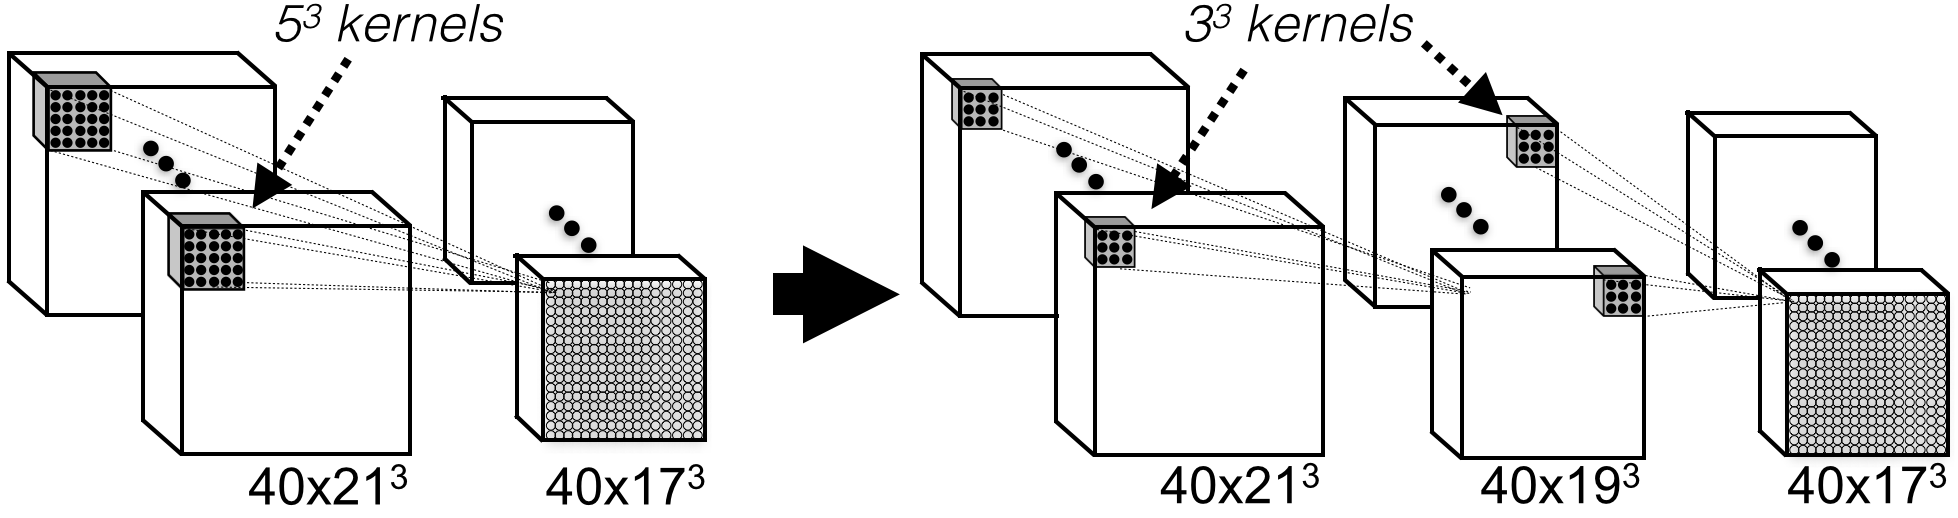
\includegraphics[clip=true, trim=0pt 0pt 0pt 0pt, width=1.0\textwidth]{figures/methodSection/deepProblems/deeper3x3.png}
\end{subfigure}

\caption{The replacement of the depicted layer with $5^5$ kernels (left) with two successive layers using $3^3$ kernels (right) introduces an additional non-linearity without altering the CNN's receptive field. Additionally, the number of weights is reduced from 200k to 86.4k and the required convolutions are cheaper (see text). Number of FMs and their size depicted as (\textit{Number $\times$ Size}).}
\label{fig:deeper3x3}
\end{figure}
%\vspace{-1pt} %takes away some white space before figure